\documentclass[a4paper]{article}

\usepackage[utf8]{inputenc}
\usepackage{indentfirst}
\usepackage{graphicx}
\usepackage{polski}
\usepackage{float}
\usepackage[left=2.5cm,right=2.5cm,top=2cm,bottom=2cm]{geometry}
\linespread{1.3}

\title{\textbf{Fractal Generator} \\ Aplikacje Internetowe i Rozproszone \\ projekt}
\author{Jakub Burzała, Krzysztof Cabała, Bartosz Cieśla, Adrian Frydmański, Dawid Gracek, Bartosz Kardas}

\usepackage{listings}
\usepackage{color}

\definecolor{mygreen}{rgb}{0,0.6,0}
\definecolor{mygray}{rgb}{0.5,0.5,0.5}
\definecolor{mymauve}{rgb}{0.58,0,0.82}

\lstset{ %
  backgroundcolor=\color{white},   % choose the background color; you must add \usepackage{color} or \usepackage{xcolor}
  basicstyle=\footnotesize,        % the size of the fonts that are used for the code
  breakatwhitespace=false,         % sets if automatic breaks should only happen at whitespace
  breaklines=true,                 % sets automatic line breaking
  captionpos=b,                    % sets the caption-position to bottom
  commentstyle=\color{mygreen},    % comment style
  deletekeywords={...},            % if you want to delete keywords from the given language
  escapeinside={\%*}{*)},          % if you want to add LaTeX within your code
  extendedchars=true,              % lets you use non-ASCII characters; for 8-bits encodings only, does not work with UTF-8
  frame=single,	                   % adds a frame around the code
  keepspaces=true,                 % keeps spaces in text, useful for keeping indentation of code (possibly needs columns=flexible)
  keywordstyle=\color{blue},       % keyword style
  language=Octave,                 % the language of the code
  otherkeywords={*,...},           % if you want to add more keywords to the set
  numbers=left,                    % where to put the line-numbers; possible values are (none, left, right)
  numbersep=5pt,                   % how far the line-numbers are from the code
  numberstyle=\tiny\color{mygray}, % the style that is used for the line-numbers
  rulecolor=\color{black},         % if not set, the frame-color may be changed on line-breaks within not-black text (e.g. comments (green here))
  showspaces=false,                % show spaces everywhere adding particular underscores; it overrides 'showstringspaces'
  showstringspaces=false,          % underline spaces within strings only
  showtabs=false,                  % show tabs within strings adding particular underscores
  stepnumber=1,                    % the step between two line-numbers. If it's 1, each line will be numbered
  stringstyle=\color{mymauve},     % string literal style
  tabsize=2,	                   % sets default tabsize to 2 spaces
  title=\lstname                   % show the filename of files included with \lstinputlisting; also try caption instead of title
}

\begin{document}

\begin{titlepage}
	\centering
	
\includegraphics[width=\textwidth]{banner2.png}\par\vspace{1cm}
	{\scshape\LARGE Politechnika Wrocławska \par}
	\vspace{1cm}
	{\scshape\Large Aplikacje Internetowe i Rozproszone\par}
	\vspace{1.5cm}
	{\huge\bfseries Generowanie fraktali z użyciem klastra obliczeniowego \par}
	\vspace{2cm}
	{\Large\itshape Jakub Burzała \\ Krzysztof Cabała \\ Bartosz Cieśla \\ Adrian Frydmański \\ Dawid Gracek \\ Bartosz Kardas \par}
	\vfill
	pod przewodnictwem\par
	dr hab. inż. Henryka \textsc{Maciejewskiego}

	\vfill

% Bottom of the page
	{\large \today\par}
\end{titlepage}

\newpage
\clearpage
\tableofcontents
\newpage

\section{Cel projektu i wymagania}
Celem projektu jest stworzenie aplikacji do generowania fraktali z użyciem technologii internetowych i zrównoleglonych obliczeń na klastrze MPI.

\textbf{Użytkownik aplikacji powinien móc:}
\begin{enumerate}
\item Wpisać dowolną funkcję zespoloną generującą fraktal
\item Zobaczyć wygenrowany fraktal
\item Przybliżyć obraz w pewnym punkcie płaszczyzny
\begin{itemize}
\item klikając
\item suwakiem
\item zaznaczając pewien obszar
\end{itemize}
\item Określić:
\begin{itemize}
\item czas trwania animacji
\item liczba klatek na sekundę
\item rozdzielczość
\end{itemize}

\item Zatrzymać, przewinąć, wznowić animację
\item Wybrać rodzaj animacji. Animowanie względem:
\begin{itemize}
\item przybliżenia -- wartość początkowa i końcowa
\item punktu centralnego (ścieżki) -- wybranie dwóch punktów na płaszczyźnie (początek i koniec) oraz zdefiniowanie ścieżki pomiędzy nimi, która wskazuje w jaki sposób będzie poruszać się kamera
\item parametrów zespolonych -- dowoloność we wprowadzaniu parametrów w równaniu zespolonym. Każdy z nich może być zmieniany z zadanym krokiem podczas animacji
\item kolorystyki -- wybór kolorystyki fraktala, definiowanie własnych zasad kolorowania
\item kroków zbieżności -- ilość maksymalnej ilość kroków zbieżności, potrzebnych do obliczenia koloru danego piksela
\end{itemize}

\item Łączyć powyższe animacje:
\begin{itemize}
\item szeregowo -- animacje odtwarzają się po sobie
\item równolegle -- animacje wykonują się w tym samym momencie
\end{itemize}

\item Zobaczyć postęp prac przy generacji animacji w postaci paska postępu oraz przewidywany czas zakończenia 
\item Zobaczyć skalę przybliżenia w postaci łatwej do wyobrażenia jednostki. Przykładowo punkt początkowy: 100 px odpowiada 1 km. W miarę prybliżania aktualizowanie jednostki do m, cm, mm itd.
\item Zapisać opis animiacji (funkcja, parametry itp) na swoje urządzenie
\item Odczytać wcześniej zapisany opis animacji
\item Zapisać animację na swoje urządzenie
\item Podzielić się wynikiem na Facebooku :)
\item Przygotowanie zadania, bez edytora tylko z pliku konfiguracyjnego
\item Logować się na serwer
\end{enumerate}
\textbf{Administrator powinien móc:}
\begin{enumerate}
\item Płynnie przełączać się pomiędzy typem prostym double, a klasą mpf implementującą liczby zmiennoprzecinkowe dowolnej dokładności
\item Wybierać metodę zrównoleglania 
\begin{itemize}
\item piksele
\item linie
\item klatki
\item części animacji
\end{itemize}
\item Wybierać liczbę jednostek wykonawczych
\end{enumerate}
\textbf{Aplikacja powinna:}
\begin{enumerate}
\item Zarządzać zadaniami, kolejkować je
\item Sekwencyjnie wykonywać zadania dla wielu użytkowników (z priorytetowaniem)
\end{enumerate}

\newpage

\section{Prototyp}
\subsection{Opis ogólny}
\begin{enumerate}
\item Przynajmniej 2 liczące slave'y
\item Może być jednoużytkownikowy system -- zlecamy zadanie i trzymamy na serwerze, żeby można było wrócić do niego po jakimś czasie.
\item Wynikiem może być wykonanie fraktala (1 klatki) lub film -- dowolność.
\item Zlecenie zadania z np. wczytywaną konfiguracją z pliku, przekazanie do serwera, zakończenie zadania i zwrócenie wyniku użytkownikowi.
\end{enumerate}
\subsection{Opis szczegółowy}
\begin{enumerate}
\item Klaster złożony z co najmniej dwóch maszyn, na każdej wykorzystywane wszystkie wątki procesora
\item Interfejs webowy umożliwiający zapamiętanie kolejki zadań
\item Możliwość pobrania wygenerowanego filmu (ew. obrazka)
\item Możliwość wpisania dowolnej funkcji zespolonej
\item Określenie czasu trwania animacji
\item Generowanie animacji na podstawie klatek kluczowych
\item Każda klatka kluczowa opisana współrzędnymi dwóch rogów obrazka
\item Wybór rozdzielczości animacji
\item Wybór między odcieniami szarości a kolorowym obrazkiem
\item Opis sceny wczytany z pliku tekstowego przygotowanego  w edytorze tekstu
\item Interfejs webowy bez podziału na użytkowników uruchomiony na komputerze z aplikacją master
\item Kolejka może być obsługiwana przez aplikację odpowiadającą za interfejs webowy
\end{enumerate}
\newpage

\section{System w wersji finalnej}
Aplikacja spełnia wymagania. Posiada czytelny interface użytkownika umożliwiający wprowadzanie nowych danych celem wykonania obliczeń. Wynikiem tychże jest animacja, której elementem jest fraktal. 
\par
Na działający serwis składa się kilka elementów. Są to:
\begin{itemize}
\item Serwer bazodanowy -- MySQL Server
\item Klaster MPI generujący animacje
\item Serwer internetowy
\end{itemize}

\subsection{Baza danych}
Baza danych służy do przesyłania zadań pomiędzy aplikacją w Django, a aplikacją rozproszoną oraz do zarządzania użytkownikami systemu. Umieszczona jest na serwerze MySQL. Poniżej widoczny jest jej model fizyczny.
 \begin{figure}[H]
    \centering
    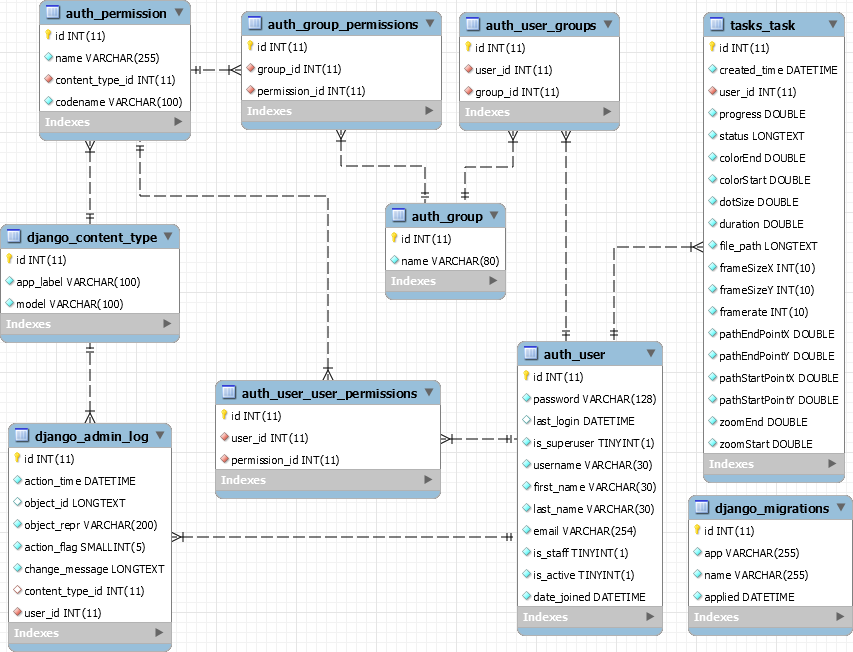
\includegraphics[width=\textwidth]{sql.png}
    \caption{Model bazy danych}
    \label{fig:db}
\end{figure}

Kluczową dla zapewnienia funkcjonalności serwisu jest tabela tasks\_task. Zawiera ona informację o zadaniach (zarówno parametry i status wykonania, jak i informację o dacie dodania i autorze). \\
Tabela auth\_user zawiera użytkowników. Te i pozostałe tabele obsługuje serwer Django, między innymi na nich opierając swoje działanie.

\subsection{MPI}
Program co ustalony kwant czasu odpytuję bazę danych, sprawdzając czy są nowe zadania do wykonania. Jeśli znajdzie takowe, zaczyna je liczyć, zaprzęgając do pracy węzły MPI.

Główna funkcja programu jest dość prosta. W zależności od roli, jaką ma pełnić program, uruchamiany jest master lub slave.
\begin{lstlisting}
#include "FractalCalc.h"
#include "Display.h"
#include "Utils.h"
#include "Comunicator.h"
#include "Master.h"
#include "Slave.h"

double zoom = 1.01;
extern bool noDisplay;

int main(int argc, char** argv) 
{
	// compareArguments(argc, argv);
	
	// MPI initialization
    MPI_Init(&argc, &argv);
    registerMPIDataTypes();
    // Get the number of processes
    int world_size;
    MPI_Comm_size(MPI_COMM_WORLD, &world_size);
    // Get the rank of the process
    int rank;
    MPI_Comm_rank(MPI_COMM_WORLD, &rank);
    if(rank == 0) 
    {
    	Master m;
        system("echo Master: $(hostname)");
    	m.work(argc, argv);
    }
    else 
    {
    	Slave s;
    	s.work(argc, argv);
    }
 
    // Finalize the MPI environment.
    MPI_Finalize();
    return 0;
}
\end{lstlisting}

\subsubsection{Master}
Master odpowiada za sprawdzanie bazy danych. 

\begin{lstlisting}
MysqlComm com(HOST, USER, PASS, DB);
try
{
	com.Init();
	com.Connect();
	do
	{
		sleep(1);
		com.Select("tasks_task","*");
		cout<<"Bool: "<<com.AnythingToDo()<<endl;
	}
	while( ! com.AnythingToDo() );
} catch(const char* e){
	printf("%s\n", e);
	fflush(stdout);
}
\end{lstlisting}

Jeśli znajdzie zadanie, pobiera jego parametry i rozsyła zadanie slave'om. Po odebraniu zadania aktualizowany jest jego status, dzięki czemu na stronie internetowej widać pasek postępu -- o którym w dalszej części dokumentacji.

\begin{lstlisting}
Task task = com.GetTask();
Scene s = com.GetScene();
com.TaskStart();
com.PrintRow();

vector<Order> orders(ordersCount);
int orderLength = generateOrders(orders, s, s.frameSize.x * s.frameSize.y / atoi(argv[1]) );

int ordersPendingCount = ordersCount;
system("echo start_tasks $(date +%X) $(($(date +%s%N)/1000000)) >> time.log");
for(int i = 1; i < world_size; ++i)
{
	sendOrder(orders[ordersCount - ordersPendingCount], i, WORKTAG);
	ordersPendingCount--;
}
map<int, vector<double>> results;
while(ordersPendingCount > 0)
{
	receiveResult(results, MPI_ANY_SOURCE);
	sendOrder(orders[orders.size() - ordersPendingCount], status.MPI_SOURCE, WORKTAG);
	ordersPendingCount--;
	int progress = 100 - (ordersPendingCount*100) / ordersCount;
	com.TaskUpdateProgress(progress);
	cout << progress << endl;
}
\end{lstlisting}

Slave'y pobierają zadania -- pojedyncze klatki do wygenerowania. Wygenerowane obrazy odbierane są od slave'ów:

\begin{lstlisting}
for(; orderID < ordersCount; ++orderID)
{
	if( orderID > 0 && (orderID % ordersPerFrame == 0) )
	{
		stringstream ss;
	 	ss<<"images/"<<(orderID / ordersPerFrame)<<".bmp";
		image.save_image(ss.str().c_str());
		cout << "IMG "<<ss.str()<<endl;
	}
	for(int i = 0; i < results[orderID].size() / 3; ++i)
	{
		r = results[orderID][3*i+0];
		g = results[orderID][3*i+1];
		b = results[orderID][3*i+2];

		image.set_pixel(x++, y, r, g, b);
		int tempX = x;
		x = tempX % s.frameSize.x;
		y = (y + (tempX / s.frameSize.x)) % s.frameSize.y;
	}
}
\end{lstlisting}

Kiedy wszystkie zadania sleve'ów zostaną wykonane, master łączy klatki w film za pomocą programu ffmpeg:

\begin{lstlisting}
stringstream ss;
ss << "ffmpeg -framerate 30 -y -i images/%d.bmp -c:v libx264 -r 30 -pix_fmt yuv420p " << task.id <<".mp4";
system(ss.str().c_str());
\end{lstlisting}

\subsubsection{Slave}
Slave jest odpowiedzialny za generowanie fraktala.

\begin{lstlisting}
void Slave::work(int &argc, char** &argv)
{
	int64_t size = 0;
	int tag = 0;
	while(doWork)
	{
		waitForOrder(order);
		doWork = order.doWork;
		size = 0;
		
		if(true == order.doWork)
		{
			size = executeOrder(order, resultArray);
			if(size > 0)
			{
				int64_t id = order.orderID;
				sendResult(id, resultArray, size);
			}
			else
				doWork = false;
		}
		else
	}
}
\end{lstlisting}

Wykonywanie zadania na poziomie slave'a odbywa się w metodzie executeOrder, a jego wynik dostępny w vectorze resultArray (polu klasy Slave).
\begin{lstlisting}
int64_t Slave::executeOrder(Order &order, vector<double> &resultArray)
{
	int64_t size = 0;
	if(order.count > 0)
	{
	    resultArray.resize(order.count);
	    size = FractalCalc::calcMandelbrotPart(resultArray.data(), order);
	    vector<double> colorArray(3*size);
	    int x = order.beginX;
	    int y = order.beginY;
	    for(int i = 0; i < order.count; ++i)
    	{
        	double color = resultArray[i];
        	double r, g, b;
    	    r = 0.5*(sin(2*M_PI*color - M_PI/2 + M_PI /3) + 1) * 255.0;
    	    g = 0.5*(sin(2*M_PI*color - M_PI/2) + 1) * 255.0;
    		b = 0.5*(sin(2*M_PI*color - M_PI/2 - M_PI / 3) + 1) * 255.0;
            colorArray[3*i + 0] = r;
            colorArray[3*i + 1] = g;
            colorArray[3*i + 2] = b;
			int tempX = ++x;
			x = tempX % order.pictureWidth;
			y = (y + (tempX / order.pictureWidth)) % order.pictureHeight;

    	}
	    resultArray.swap(colorArray);
	    size = resultArray.size();
	}
    return size;
}
\end{lstlisting}

\subsubsection{Mandelbrot -- generowanie fraktala}
Slave wywołuje metodę liczącą fraktal -- calcMandelbrotPart -- z klasy FractalCalc.
\begin{lstlisting}
class FractalCalc
{
public:
	typedef void (* FractalFnPtrD)(complex<double>&, complex<double>&);
	static const int convergenceSteps;
	static const double divergenceLimitD;
	//double
	static void mandelbrotFractal(complex<double> &z, complex<double> &c);
	static double getConvergence(double z_real, double z_imag, double c_real, double c_imag, FractalFnPtrD fn);
	static int calcMandelbrotPart(double* mandelbrot, Order &order);
};

void FractalCalc::mandelbrotFractal(complex<double> &z, complex<double> &c)
{
	z = z * z + c;
}

double FractalCalc::getConvergence(double z_real, double z_imag, double c_real, double c_imag, FractalFnPtrD fn)
{
	complex<double> z(z_real, z_imag);
	complex<double> c(c_real, c_imag); // c_real => c(e)real xD

	// Sprawdzanie zbieznosci
	int j = 0;
	for (; j < convergenceSteps && abs(z) < divergenceLimitD; j++)
	{
		fn(z, c);
	}
	double log_zn, nu, result;
	if ( j < convergenceSteps ) 
	{
		log_zn = log( abs(z) );
		nu = log( log_zn / log(2) ) / log(2);
		result = (j + 1 - nu) / convergenceSteps;
	}
	return result;
}

int FractalCalc::calcMandelbrotPart(double* mandelbrot, Order &order)
{
	int iX = order.beginX;
	int iY = order.beginY;
	int i = 0;
	for (; i < order.count; ++i, ++iX)
	{
		if(iX >= order.pictureWidth)
		{
			iX = 0;
			++iY;
		}
		double dX = (order.fractalX - order.pictureWidth/2 * order.dotSize) + order.dotSize*iX;
		double dY = (order.fractalY - order.pictureHeight/2 * order.dotSize) + order.dotSize*iY;
		mandelbrot[i] = getConvergence(0, 0, dX, dY, mandelbrotFractal);
	}
	return i;
}
\end{lstlisting}


\subsection{Django}
Aplikacja napisana z użyciem frameworku Django jest kolejnym ważnym elementem systemu. To ona odpowiada za komunikację użytkownik -- baza danych.

Widoki dostępne w interfejsie użytkownika, to strona główna, logowanie, rejestracja, dodawanie nowego fraktala i przeglądanie już dodanych w postaci wygenerowanych animacji. Poniżej umieszczono przykładowy szablon strony głównej i strony Moje animacje:

\begin{lstlisting}

<!DOCTYPE html>
<head>
<meta http-equiv="Content-Type" content="text/html; charset=utf-8" />
<title>{{ site.name }}</title>
<meta name="keywords" content="" />
<meta name="description" content="" />
<link href="http://fonts.googleapis.com/css?family=Varela" rel="stylesheet" />
<link href="" rel="stylesheet" />
<link href="" rel="stylesheet" />
<!--
<script src="//code.jquery.com/jquery-1.11.1.min.js"></script>
<script src=""></script>
-->
<!--[if IE 6]><link href="" rel="stylesheet" type="text/css" /><![endif]-->
</head>
<body>
<div id="wrapper">
	<div id="header-wrapper">
		<div id="header" class="container">
			<div id="logo">
				<h2><a href="">FRACTAL<br />GENERATOR</a></h2>
			</div>
            
            
		</div>
	</div>
	<div id="extra" class="container">
        
            
                
                
            
        
        
		    
            
        
	</div>
</div>
<div id="copyright" class="container">
	<p>&copy; Untitled. All rights reserved. | Photos by <a href="http://fotogrph.com/">Fotogrph</a> | Design by <a href="http://templated.co" rel="nofollow">TEMPLATED</a>.</p>
</div>
</body>
</html>
\end{lstlisting}

\begin{lstlisting}



    <div id="menu">
				<ul>
					<li><a href="" accesskey="1" title="">Strona glowna</a></li>
                    
					    <li><a href="" accesskey="2" title="">Generuj fraktal</a></li>
					    <li><a href="" accesskey="3" title="">Moje fraktale</a></li>
					    <li class="current_page_item"><a href="" accesskey="4" title="">Moje animacje</a></li>
					    <li><a href="" accesskey="5" title="">Wyloguj</a></li>
                    
                        <li><a href="" accesskey="2" title="">Zaloguj</a></li>
                    
				</ul>
			</div>


    <h1>Moje Animacje</h1>
    <br /><br />
    
        
            <h3>{{ forloop.counter }}.&nbsp&nbsp&nbsp{{ video.created_time }}</h3>
            <video width="320" height="240" controls>
                <source src="{{  video.file_path }}" type="video/mp4">
                Your browser does not support the video tag.
            </video>
        
    
        Nie znaleziono zadnych animacji wygenerowanych przez Ciebie.
    
    <script src="//code.jquery.com/jquery-1.11.1.min.js"></script>
<script src=""></script>


    <h1>Strona Glowna</h1>
    Zaloguj sie aby rozpoczac korzystanie z serwisu. Jezeli nie masz jeszcze konta <a href="">zarejestruj sie!</a>

\end{lstlisting}

Formularz rejestracji generuje Django.
\begin{lstlisting}




        <form method="post" action=".">
            
            {{ form.as_p }}
            <label>&nbsp;</label><input type="submit" value=""/>
        </form>

\end{lstlisting}

Poniżej widoczne są przykładowe kody w Pythonie.\\
Widoki w pliku views.py:
\begin{lstlisting}
from django.shortcuts import redirect, render
from django.contrib.auth.decorators import login_required
from .forms import AddTaskForm
from .models import Task

def get_dotsize(value):
    return 4.0 / value

def index(request):
    if request.user.is_authenticated():
        tasks = Task.objects.filter(user=request.user).order_by('-created_time')
        return render(request, 'tasks/tasks.html', {'tasks': tasks})
    else:
        return render(request, 'tasks/tasks.html', {})

@login_required(login_url='/')
def add(request):
    if request.method == "POST":
        form = AddTaskForm(request.POST)
        if form.is_valid():
            post = form.save(commit=False)
            post.user = request.user
            post.dotSize = get_dotsize(post.frameSizeX)
            post.save()
            return redirect('/', pk=post.pk)
    else:
        form = AddTaskForm()
    return render(request, 'tasks/addTask.html', {'form': form})

@login_required(login_url='/')
def delete(request, task_id):
    Task.objects.filter(user_id=request.user.id, id=task_id).delete()
    return redirect('/')

@login_required(login_url='/')
def fractals(request):
    return render(request, 'tasks/fractals.html', {})

@login_required(login_url='/')
def animations(request):
    if request.user.is_authenticated():
        tasks = Task.objects.filter(user=request.user, status='done').order_by('-created_time')
        return render(request, 'tasks/animations.html', {'videos': tasks})
    else:
        return render(request, 'tasks/animations.htmll', {})
\end{lstlisting}

Plik z ustawieniami wygląda następująco:
\begin{lstlisting}
import os

# Build paths inside the project like this: os.path.join(BASE_DIR, ...)
BASE_DIR = os.path.dirname(os.path.dirname(os.path.abspath(__file__)))

# SECURITY WARNING: keep the secret key used in production secret!
SECRET_KEY = '6=saxft6ij11khby3r@((*u*frkyo9e5c!49_=!sd0k64f1qp&'

# SECURITY WARNING: don't run with debug turned on in production!
DEBUG = True

ALLOWED_HOSTS = []

# Application definition

INSTALLED_APPS = [
    'tasks.apps.TasksConfig',
    'django.contrib.admin',
    'django.contrib.auth',
    'django.contrib.contenttypes',
    'django.contrib.sessions',
    'django.contrib.messages',
    'django.contrib.staticfiles',
]

MIDDLEWARE_CLASSES = [
    'django.middleware.security.SecurityMiddleware',
    'django.contrib.sessions.middleware.SessionMiddleware',
    'django.middleware.common.CommonMiddleware',
    'django.middleware.csrf.CsrfViewMiddleware',
    'django.contrib.auth.middleware.AuthenticationMiddleware',
    'django.contrib.auth.middleware.SessionAuthenticationMiddleware',
    'django.contrib.messages.middleware.MessageMiddleware',
    'django.middleware.clickjacking.XFrameOptionsMiddleware',
]

ROOT_URLCONF = 'mandelbrot.urls'

TEMPLATES = [
    {
        'BACKEND': 'django.template.backends.django.DjangoTemplates',
        'DIRS': [],
        'APP_DIRS': True,
        'OPTIONS': {
            'context_processors': [
                'django.template.context_processors.debug',
                'django.template.context_processors.request',
                'django.contrib.auth.context_processors.auth',
                'django.contrib.messages.context_processors.messages',
            ],
        },
    },
]

WSGI_APPLICATION = 'mandelbrot.wsgi.application'

# Database
# https://docs.djangoproject.com/en/1.9/ref/settings/#databases

DATABASES = {
    'default': {
        'ENGINE': 'django.db.backends.mysql',
        'NAME': 'mandel',
        'HOST': 'adres.bazy.com',
        'PORT': '3306',
        'USER': 'mandelbrot',
        'PASSWORD': 'haslodobazy',
    }
}

# Password validation
# https://docs.djangoproject.com/en/1.9/ref/settings/#auth-password-validators

AUTH_PASSWORD_VALIDATORS = [
    {
        'NAME': 'django.contrib.auth.password_validation.UserAttributeSimilarityValidator',
    },
    {
        'NAME': 'django.contrib.auth.password_validation.MinimumLengthValidator',
    },
    {
        'NAME': 'django.contrib.auth.password_validation.CommonPasswordValidator',
    },
    {
        'NAME': 'django.contrib.auth.password_validation.NumericPasswordValidator',
    },
]

# Internationalization
# https://docs.djangoproject.com/en/1.9/topics/i18n/

LANGUAGE_CODE = 'pl-pl'

TIME_ZONE = 'Europe/Warsaw'

USE_I18N = True

USE_L10N = True

USE_TZ = True

# Static files (CSS, JavaScript, Images)
# https://docs.djangoproject.com/en/1.9/howto/static-files/

STATIC_ROOT = "/root/mandelbrot/static/"
STATIC_URL = '/static/'
STATICFILES_DIRS = (
    os.path.join("videos", "/home/dave/"),
)

REGISTRATION_OPEN = True  # If True, users can register
ACCOUNT_ACTIVATION_DAYS = 7  # One-week activation window; you may, of course, use a different value.
REGISTRATION_AUTO_LOGIN = False  # If True, the user will be automatically logged in.
LOGIN_REDIRECT_URL = '/'  # The page you want users to arrive at after they successful log in
LOGIN_URL = '/accounts/login/'  # The page users are directed to if they are not logged in,
# and are trying to access pages requiring authentication

EMAIL_USE_TLS = True
EMAIL_HOST = 'smtp.gmail.com'
EMAIL_PORT = 587
EMAIL_HOST_USER = 'fractalgenerator@gmail.com'
EMAIL_HOST_PASSWORD = 'haslodokontapocztowego'
\end{lstlisting}

Obsługa formularza:
\begin{lstlisting}
from django import forms
from .models import Task

class AddTaskForm(forms.ModelForm):
    framerates = (
         ('24', '24'),
         ('30', '30'),
         ('60', '60'),
    )

    frameSizeX = forms.IntegerField(required=True, label="Szerokosc")
    frameSizeY = forms.IntegerField(required=True, label="Dlugosc")
    framerate = forms.ChoiceField(choices=framerates, required=True, label="Liczba klatek/sekunde")
    duration = forms.FloatField(required=True, label="Czas Trwania", help_text="(s)")
    pathStartPointX = forms.FloatField(required=True, label="Punkt Startowy X")
    pathStartPointY = forms.FloatField(required=True, label="Punkt Startowy Y")
    pathEndPointX = forms.FloatField(required=True, label="Punkt Koncowy X")
    pathEndPointY = forms.FloatField(required=True, label="Punkt Koncowy Y")
    zoomStart = forms.FloatField(required=True, min_value=1, label="Powiekszenie startowe")
    zoomEnd = forms.FloatField(required=True, min_value=1, label="Powiekszenie koncowe")
    # colorStart = forms.FloatField()
    # colorEnd = forms.FloatField()

    class Meta:
        model = Task
        exclude = ['dotSize', 'progress', 'user', 'file_path', 'status', 'created_time', '', 'colorStart', 'colorEnd']
\end{lstlisting}

Zadanie:
\begin{lstlisting}
from django.db import models
from django.contrib.auth.models import User
from django.utils import timezone

class Task(models.Model):
    user = models.ForeignKey(User, on_delete=models.CASCADE, )
    created_time = models.DateTimeField(default=timezone.now, )
    file_path = models.TextField(default="", )
    status = models.TextField(default="pending", )
    progress = models.FloatField(default="0", )
    duration = models.FloatField(default="0",)
    framerate = models.PositiveIntegerField(default="0")
    frameSizeX = models.PositiveIntegerField(default="0")
    frameSizeY = models.PositiveIntegerField(default="0")
    dotSize = models.FloatField(default="0")
    pathStartPointX = models.FloatField(default="0")
    pathStartPointY = models.FloatField(default="0")
    pathEndPointX = models.FloatField(default="0")
    pathEndPointY = models.FloatField(default="0")
    zoomStart = models.FloatField(default="0")
    zoomEnd = models.FloatField(default="0")
    colorStart = models.FloatField(default="0")
    colorEnd = models.FloatField(default="0")

def get_dotsize(self):
    return 4.0 / self.frameSizeX
\end{lstlisting}

\subsection{Strona internetowa -- interfejs użytkownika}
Poniższe zrzuty ekranu prezentują działanie serwisu:
 \begin{figure}[H]
    \centering
    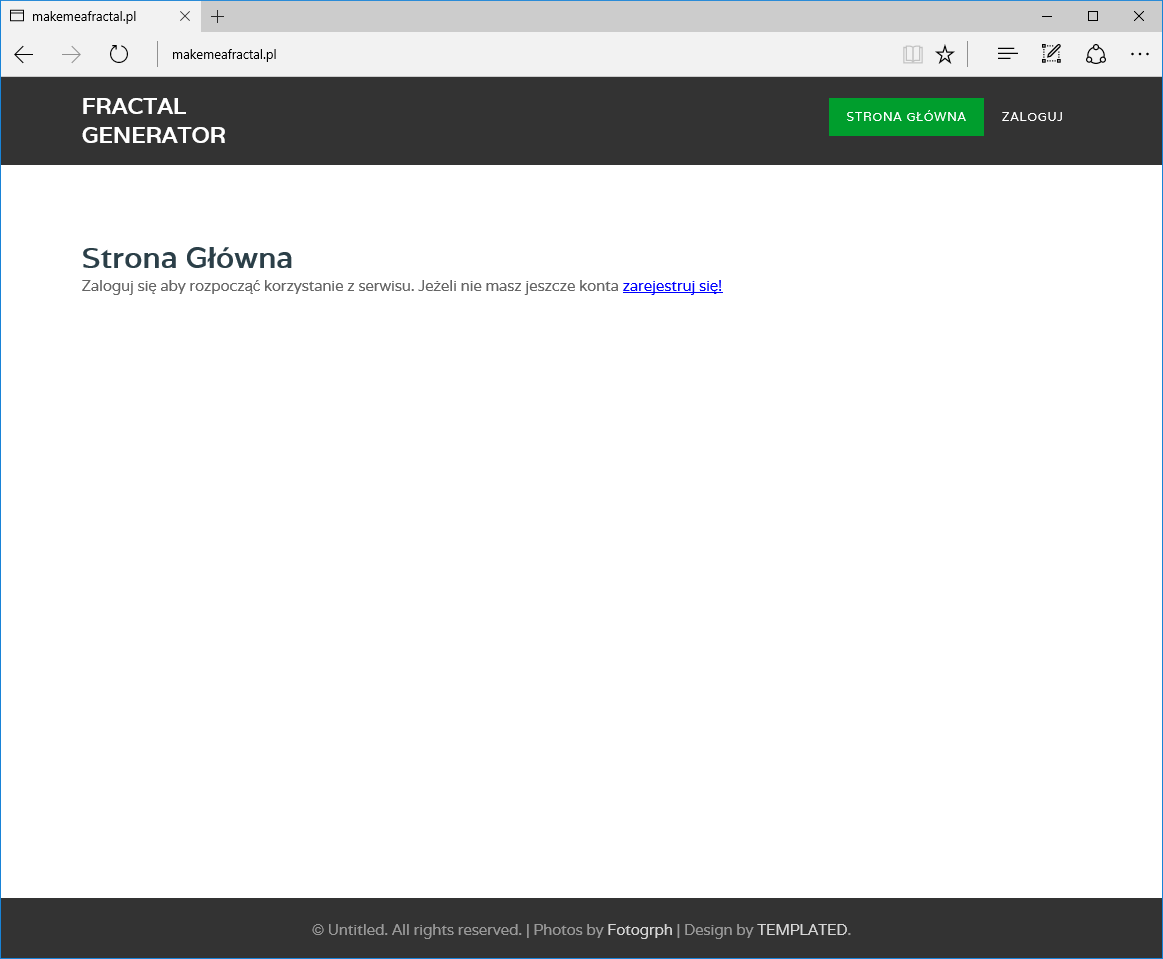
\includegraphics[width=\textwidth]{main_page.png}
    \caption{Strona główna}
    \label{fig:main_page}
\end{figure}
Na stronie głównej widoczna jest propozycja zalogowania się, lub rejestracji. Bez tego niemożliwe jest wysyłanie zadań do wykonania. 
\begin{figure}[H]
    \centering
    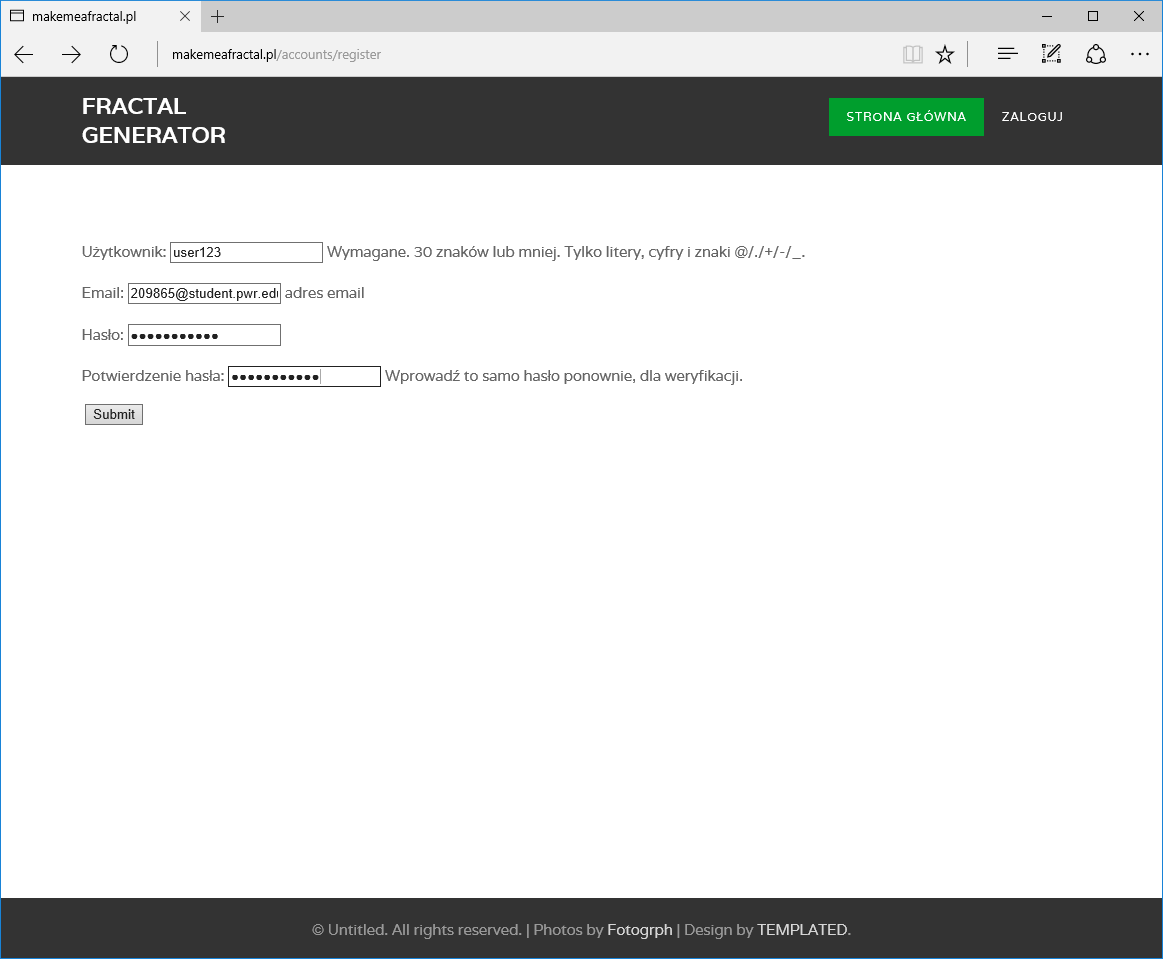
\includegraphics[width=\textwidth]{register_page.png}
    \caption{Rejestracja}
    \label{fig:reg_page}
\end{figure}
Rejestracja wymaga podania nazwy użytkownika, adresu email i hasła. Na podany adres zostaje wysłany link aktywacyjny, po kliknięciu którego można korzystać z serwisu.
\begin{figure}[H]
    \centering
    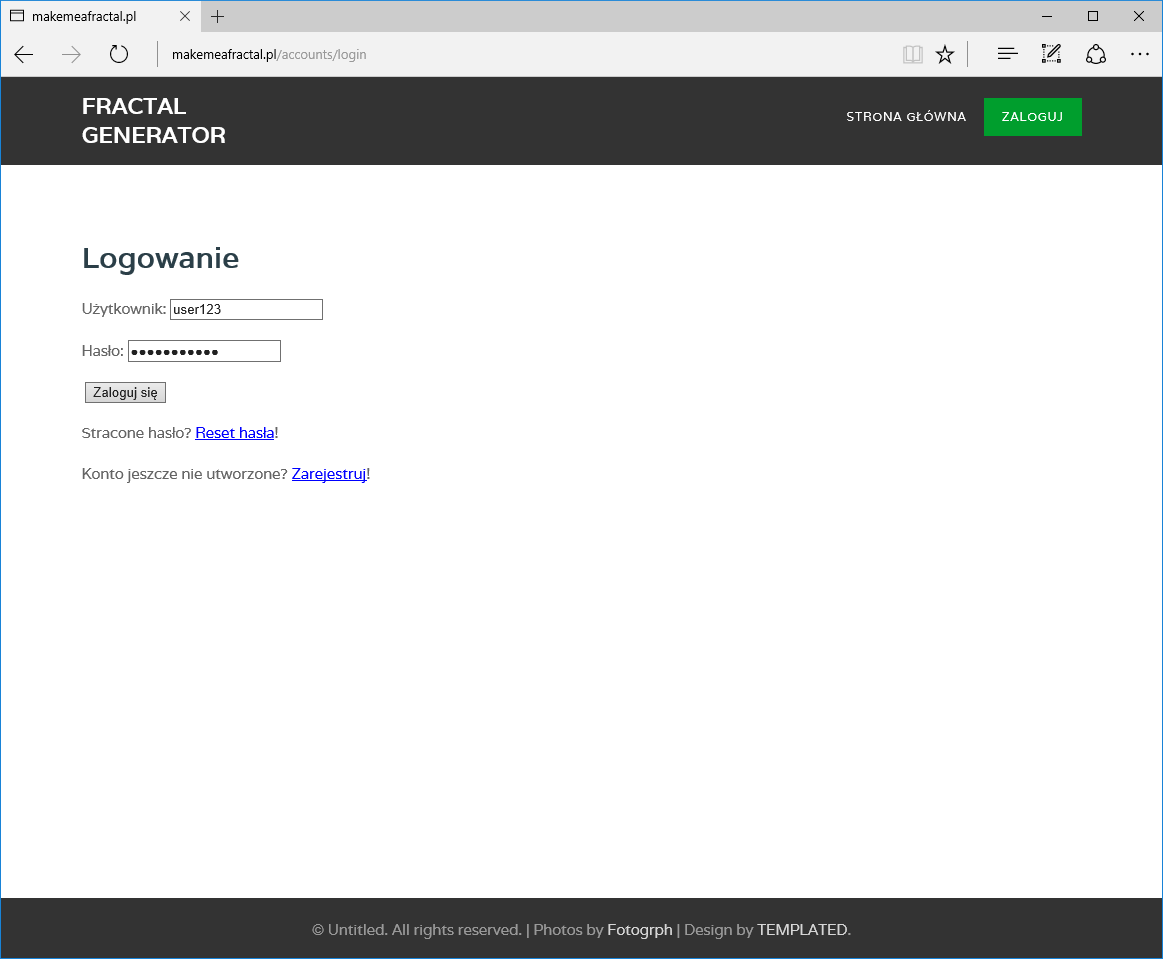
\includegraphics[width=\textwidth]{login_page.png}
    \caption{Logowanie}
    \label{fig:activ_page}
\end{figure}
\begin{figure}[H]
    \centering
    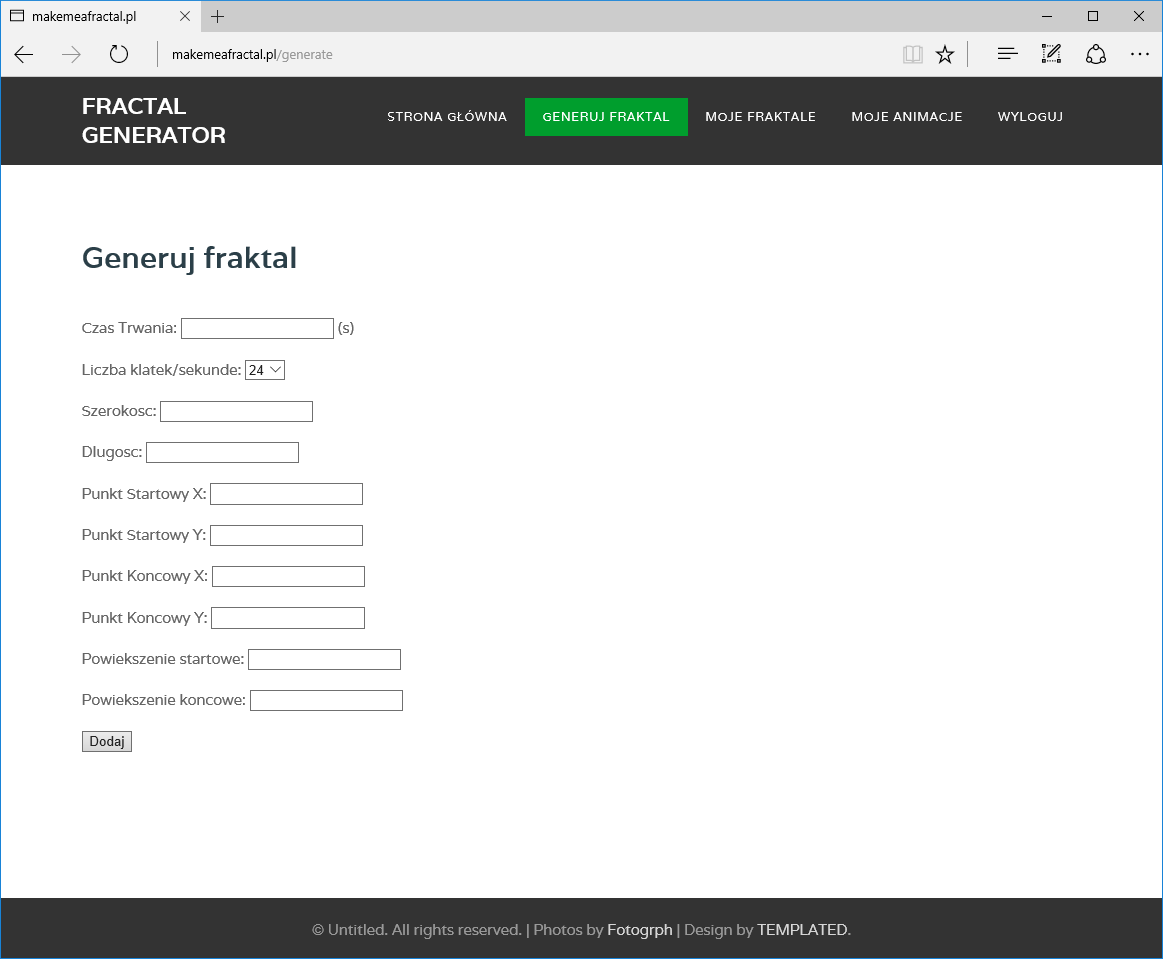
\includegraphics[width=\textwidth]{gen_page.png}
    \caption{Generowanie fraktala}
    \label{fig:gen_page}
\end{figure}
Na tej stronie istnieje możliwość dodania nowego zadania do wykonania. Podawane są parametry animacji - dotyczące zarówno pliku wideo, jak i samego fraktala i jego pozycji.
\begin{figure}[H]
    \centering
    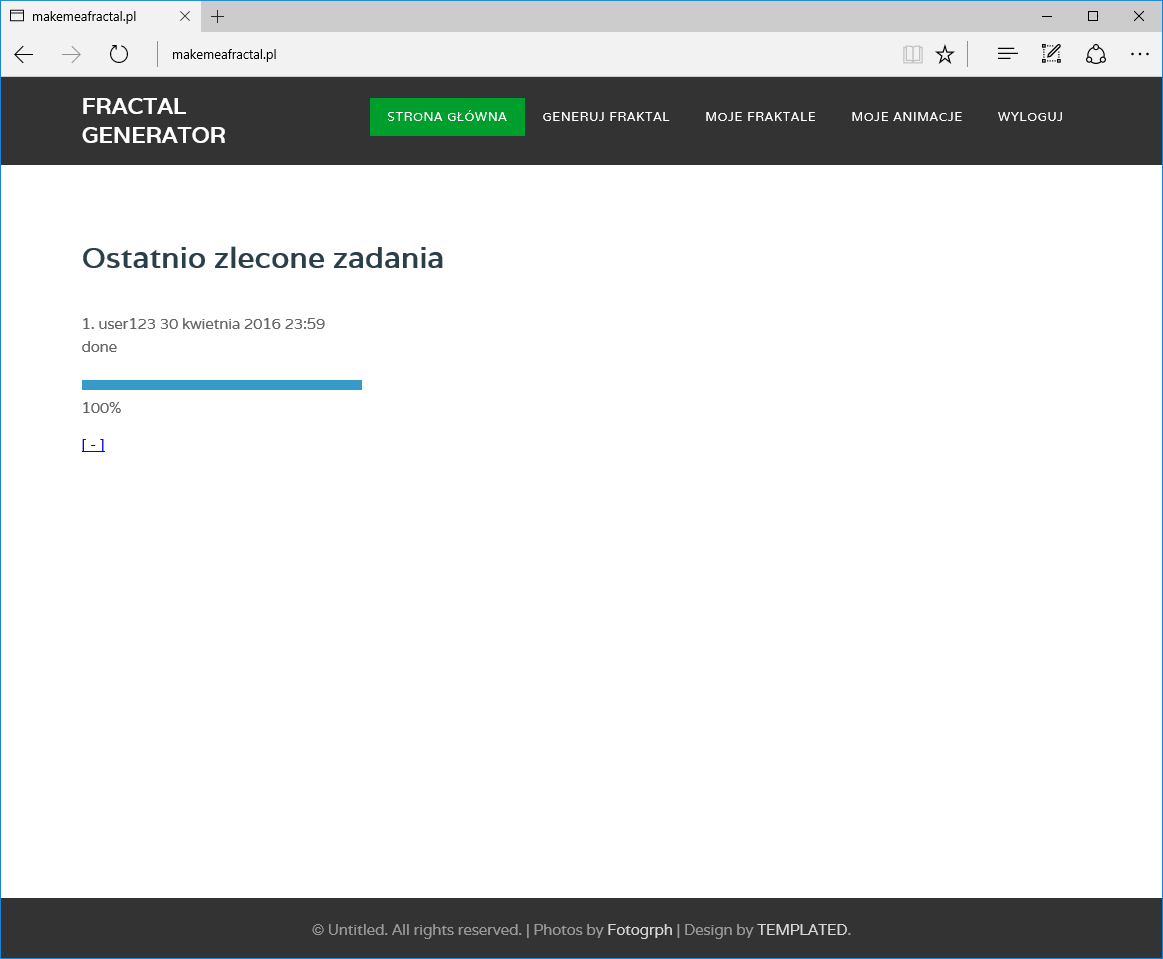
\includegraphics[width=\textwidth]{queue_page.png}
    \caption{Kolejka zadań}
    \label{fig:queue_page}
\end{figure}
Po zalogowaniu się na stronie głównej widoczne są zlecone zadania i ich status wykonania wraz z paskiem postępu.
\begin{figure}[H]
    \centering
    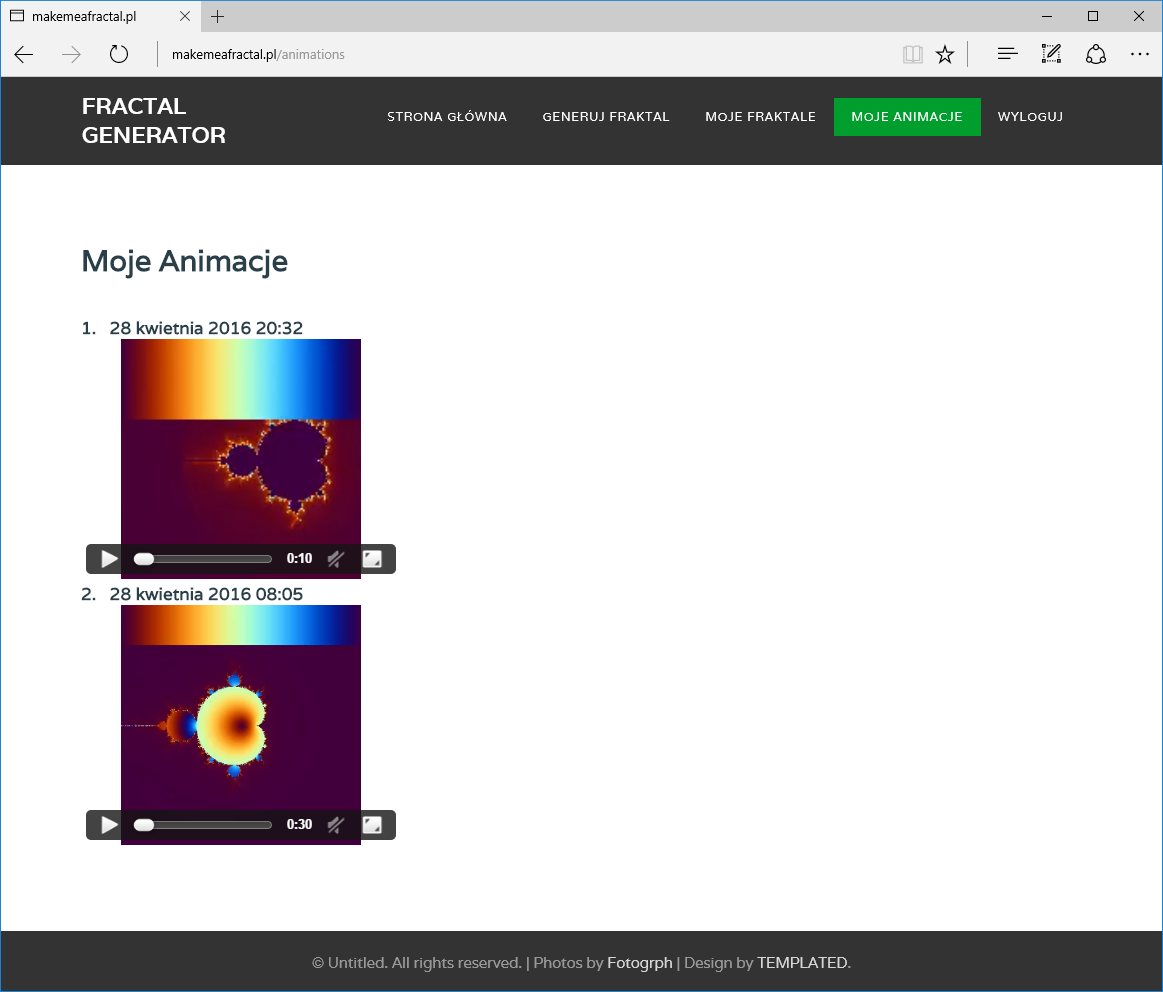
\includegraphics[width=\textwidth]{my_frac.png}
    \caption{Moje animacje}
    \label{fig:my_frac}
\end{figure}
Na stronie Moje animacje widoczny jest podgląd wygenerowanych animacji.

\newpage

\section{Uruchamianie}
W celu uruchomienia aplikacji potrzebne są następujące składniki:
\begin{itemize}
\item lib mysql
\item libctdc++6
\item serwer ssh
\item authorizedkeys
\item rsync
\item openmpi
\end{itemize}

Program obsługujący MPI znajduje się w katalogu Cluster. Należy skompilować go poleceniem make. Model bazy danych (Doc/mandel.mvb) należy otworzyć za pomocą programu MySQL Workbench i na jego podstawie wypełnić bazę tabelami. Aplikacja internetowa znajduje się w katalogu WebApp.

\section{Testy wydajności}
Testy zostały wykonane przy użyciu trzech fizycznych maszyn. 2 z nich były wyposażone w 2 (Intel i5), a jedna 4 (Intel i7) rdzenie procesora. Zastosowana w nich technologia HyperTreading pozwala na jednoczesną pracę dwóch wątków na jednym rdzeniu, zatem można stwierdzić, że były dostępne odpowiednio 4 i 8 rdzeni Maszyna na której uruchamiany był master pracowała pod kontrolą systemu operacyjnego Linux Mint, natomiast na pozostałych były zainstalowane maszyny wirtualne z systemem Linux Debian. Komputery były spięte do jednego switcha z portami FastEthernet. Dostępny sprzęt pozwolił przetestować następujące konfiguracje:
\begin{enumerate}
\item 1 maszyna fizyczna, 4 rdzenie
\item 1 maszyna fizyczna, 8 rdzeni
\item 2 maszyny fizyczne, 8 rdzeni (4 + 4)
\item 2 maszyny fizyczne, 12 rdzeni (4 + 8)
\item 3 maszyny fizyczne, 12 rdzeni (4 + 4 + 4)
\item 3 maszyny fizyczne, 16 rdzeni (4 +4 +8)
\end{enumerate}

Na wszystkich maszynach zostało uruchomione zadanie wygenerowania 1-sekundowej animacji (30 klatek) w różnej rozdzielczości (400x400 – 2000x2000 px ze skokiem co 200 px). Drugi scenariusz testowy dotyczył podziału klatki na mniejsze podzadania. W tym przypadku rozdzielczość została ustalona na 2000 x 2000 px, natomiast klatka była dzielona na 1, 2, 4, 8, 16 podzadań (seed). Wszystkie pomiary zostały wykonane 10-krotnie, a następnie uśredniono wyniki. Widoczny na wykresach przypadek all dotyczył czasu wykonania całego zadania, wraz z generowaniem animacji z gotowych klatek, natomiast mpi dotyczy wyłącznie czasu obliczeń zrównoleglonych. Wykresy na których nie ma tego podziału pokazują czasy tylko obliczeń zrównoleglonych.

\begin{figure}[H]
    \centering
    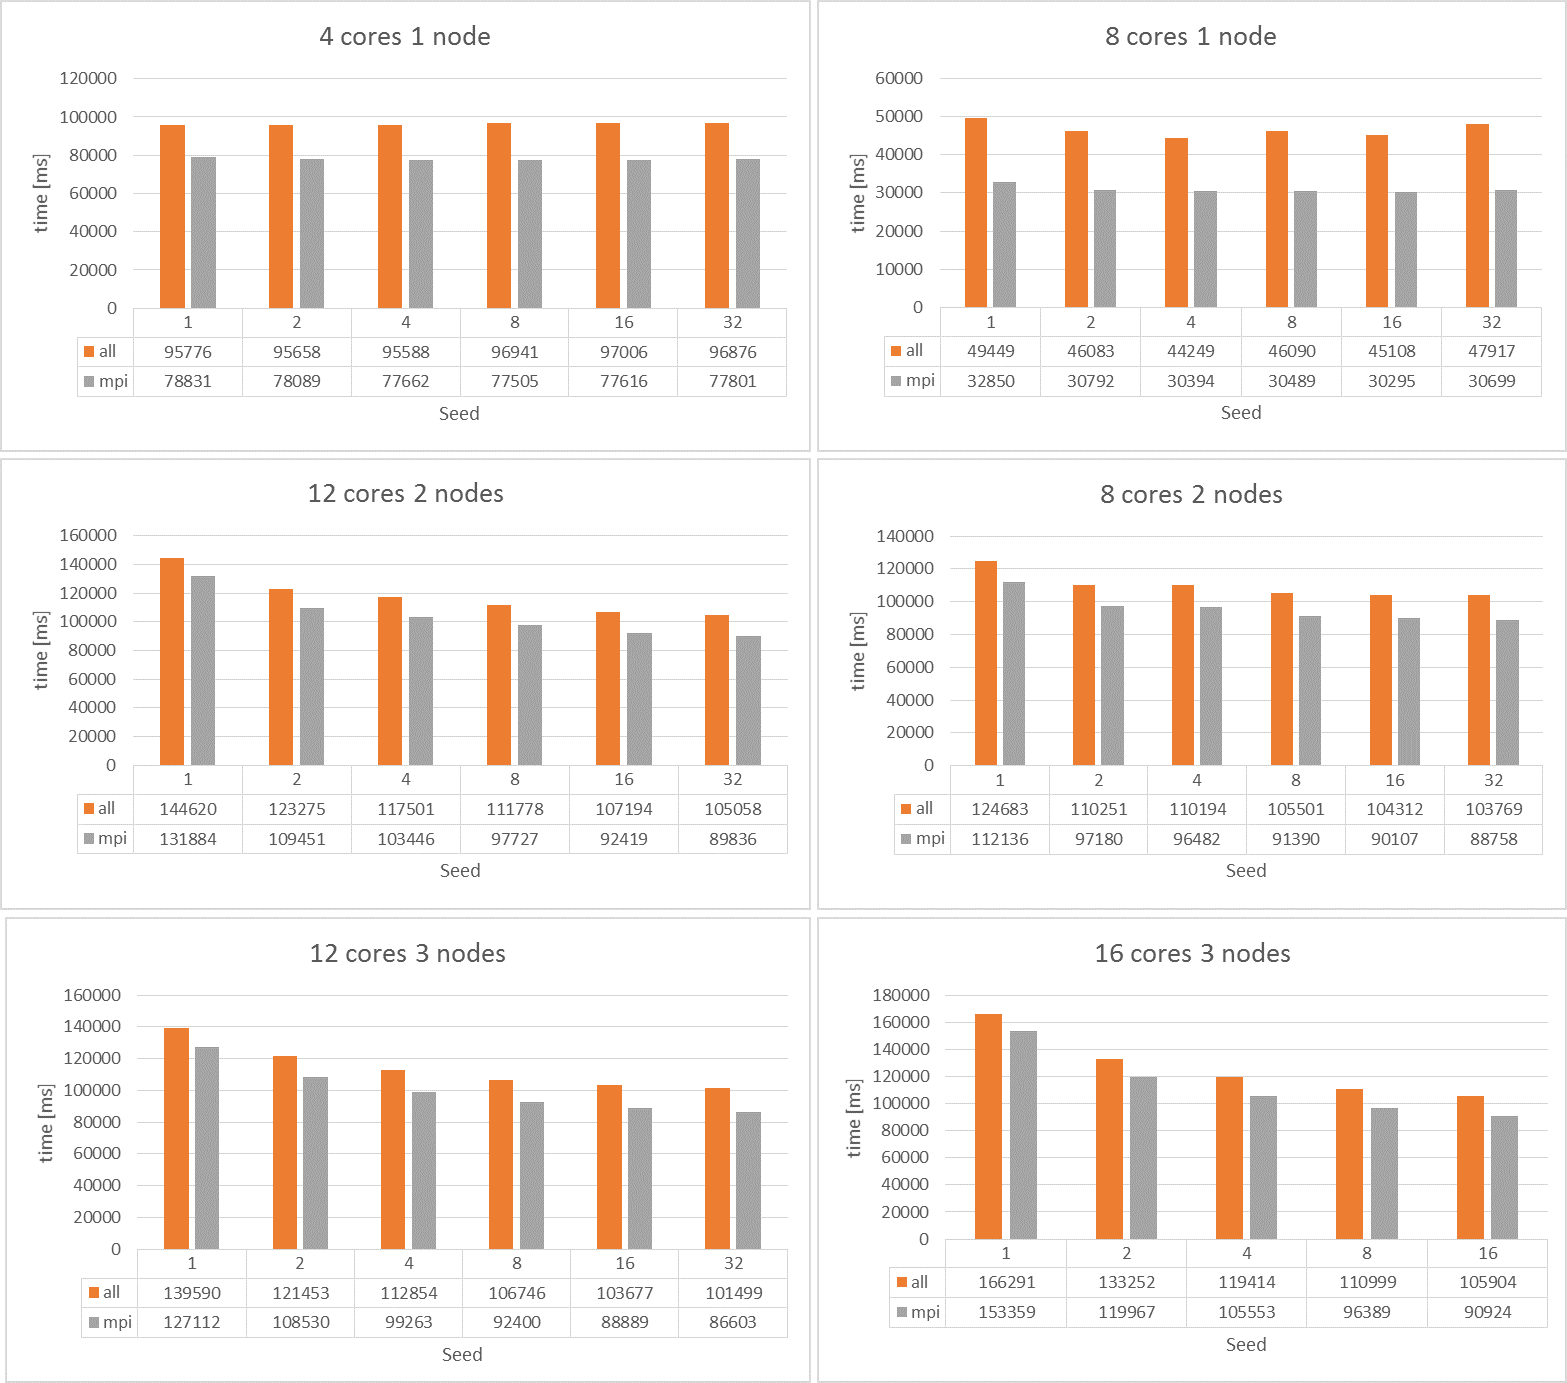
\includegraphics[width=\textwidth]{1.png}
    \caption{Porównanie czasu dla różnych konfiguracji}
    \label{fig:w1}
\end{figure}

Z powyższych wykresów widać, że jeśli wszystkie rdzenie liczące znajdują się na jednej maszynie to podział zadania na różne fragmenty nie ma większego wpływu na czas obliczeń. Jeżeli jednak zwiększymy ilość maszyn liczących, to podział zadania na mniejsze pozwala zaobserwować spadek czasu obliczeń. Różnica ta zwiększa się wraz z dokładaniem do klastra kolejnych maszyn. Również liczba przydzielonych rdzeni procesora ma znaczący wpływ na szybkość omawianej zmiany.

\begin{figure}[H]
    \centering
    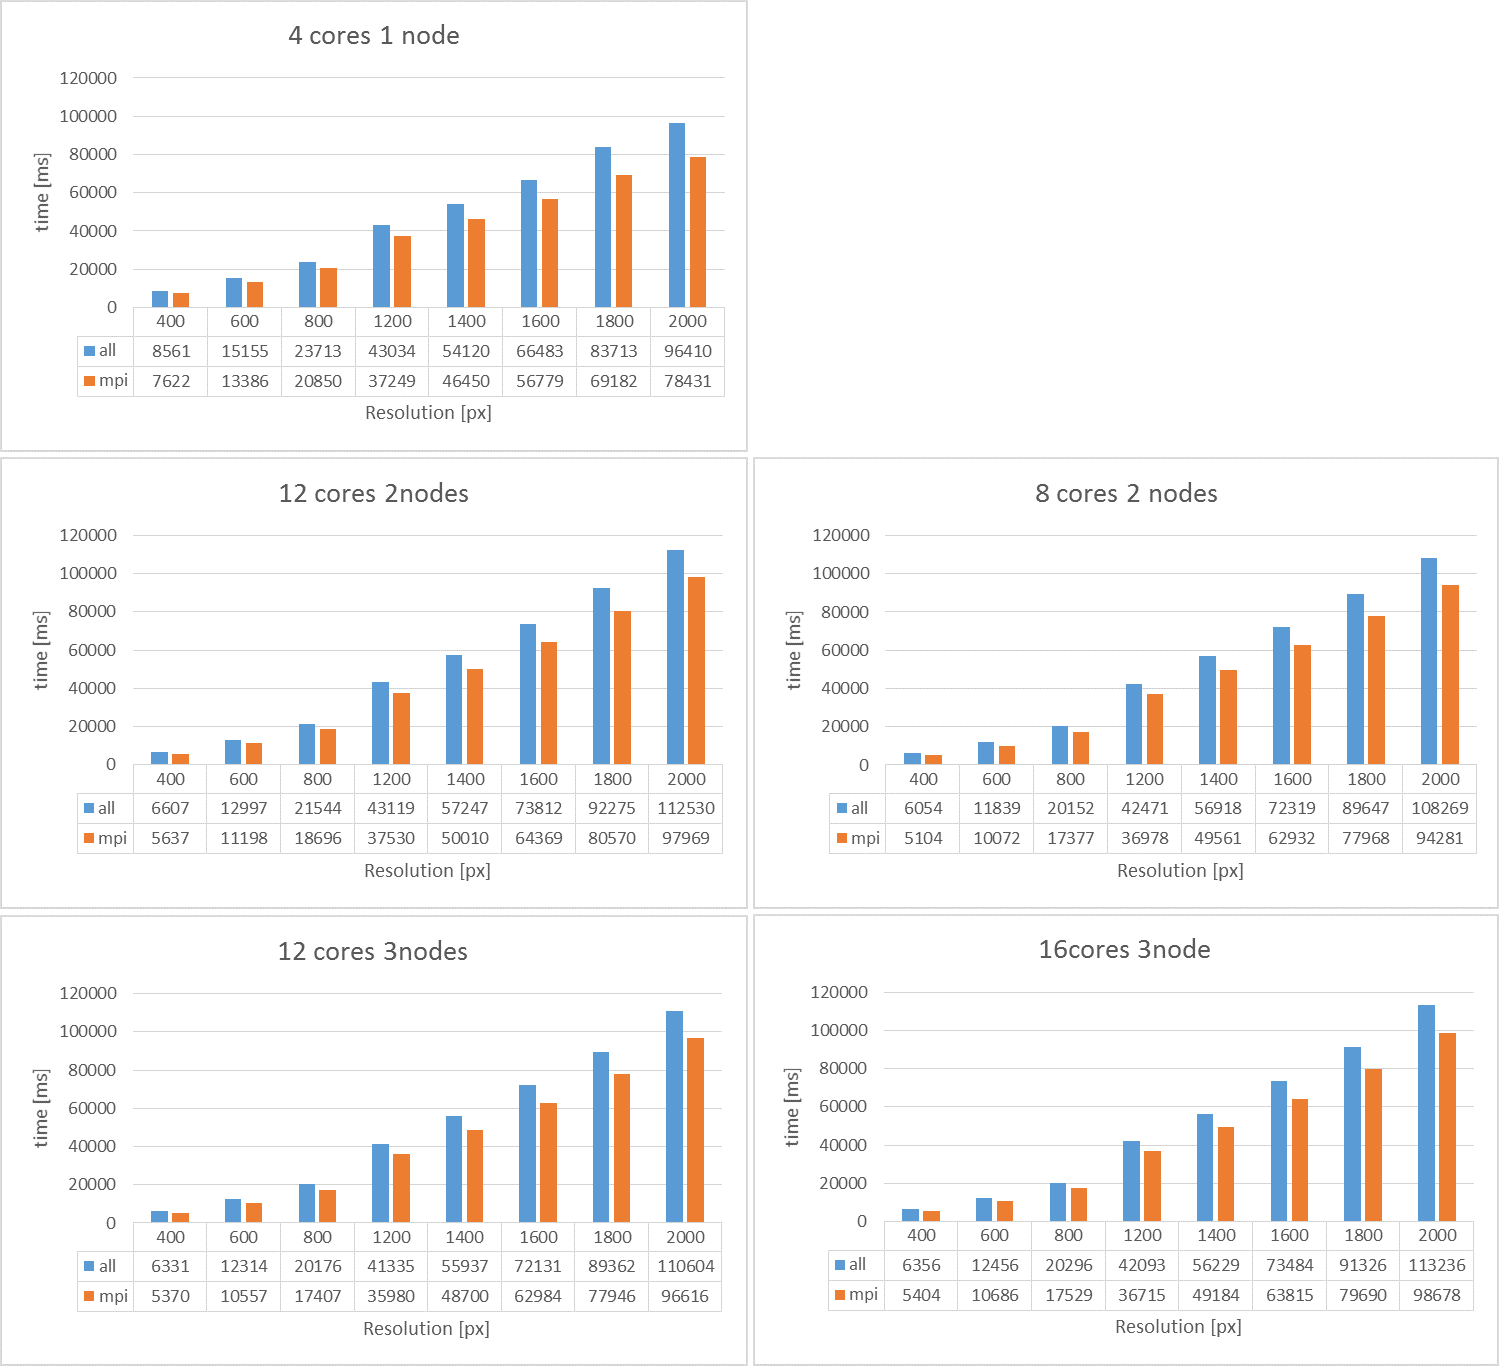
\includegraphics[width=\textwidth]{2.png}
    \caption{Porównanie czasu dla różnych rozdzielczości}
    \label{fig:w2}
\end{figure}

Porównanie czasu obliczeń w zależności od rozmiaru klatki obrazu ukazuje wyniki zgodne z oczekiwaniami. Ilość maszyn liczących i rdzeni procesora nią ma wpływu na charakter zmiany czasu obliczeń. We wszystkich przetestowanych przypadkach jest to zależność wielomianowa, zbliżona do funkcji kwadratowej. Ma to uzasadnienie w zmianie rozmiarze zadania – dwukrotne zwiększenie boku klatki powoduje czterokrotne zwiększenie rozmiaru zadania.

\begin{figure}[H]
    \centering
    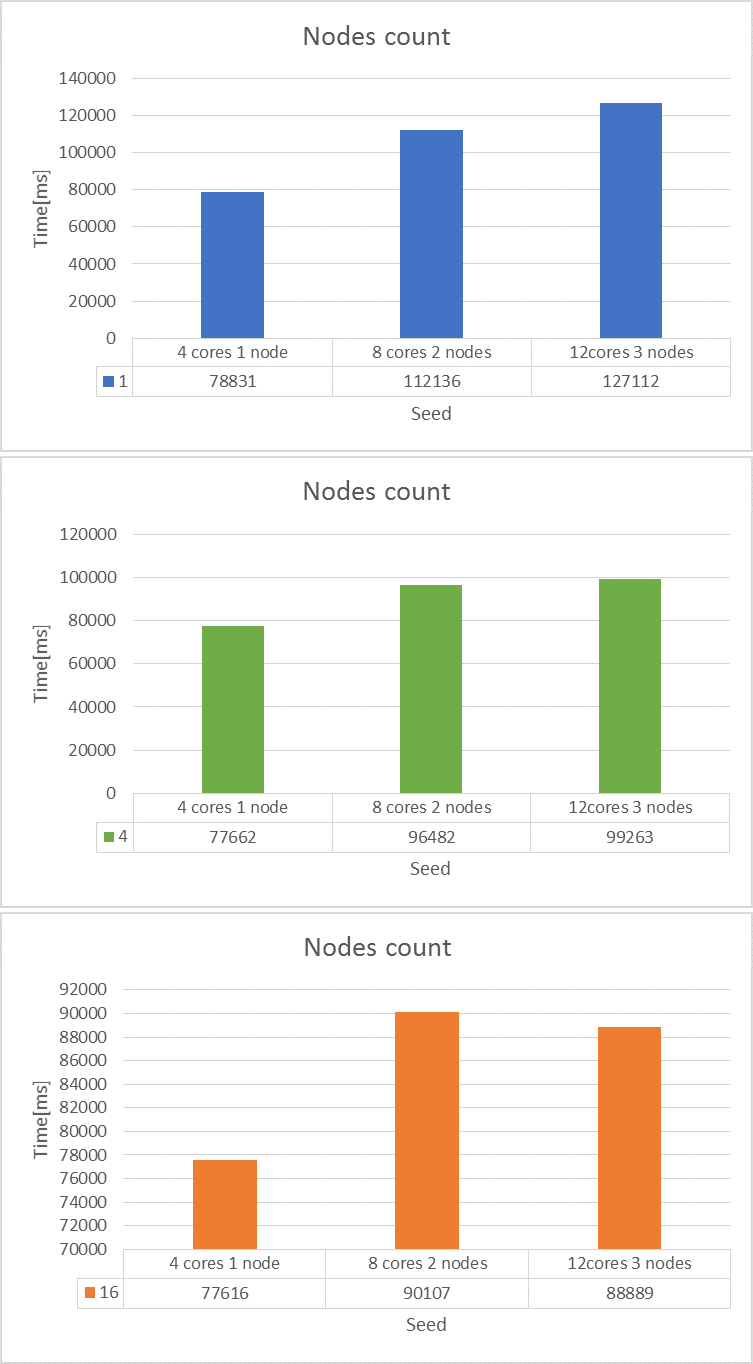
\includegraphics[width=0.5\textwidth]{3.png}
    \caption{Porównanie czasu dla różnych liczb podzadań}
    \label{fig:my_frac}
\end{figure}

Na wszystkich wykresach można zaobserwować wzrost czasu trwania wykonania zadania zależnie od ilości połączonych węzłów. Jest to spowodowane narzutem komunikacji pomiędzy węzłem master a wszystkimi węzłami slave. Patrząc jednak na wielkość ziarna zadania, czyli podziału jednej klatki na kolejno 1, 4 i 16 podzadań można zauważyć, że większe rozdrobnienie idzie w parze z przyspieszeniem czasu wykonania całości zadania, jest to lepiej widoczne im więcej węzłów połączymy ze sobą. Większa ziarnistość powoduje zmniejszenie zużycia łącza na przesłanie dużego fragmentu danych (przy ziarnie 1 przesyłana jest cała klatka, a przy 16 tylko 1/16). Przesyłanie trwa na tyle krótko żeby nie doszło do zbyt długiego blokowania węzła master podczas gdy inne węzły slave czekają na swoją kolej obsługi.

\begin{figure}[H]
    \centering
    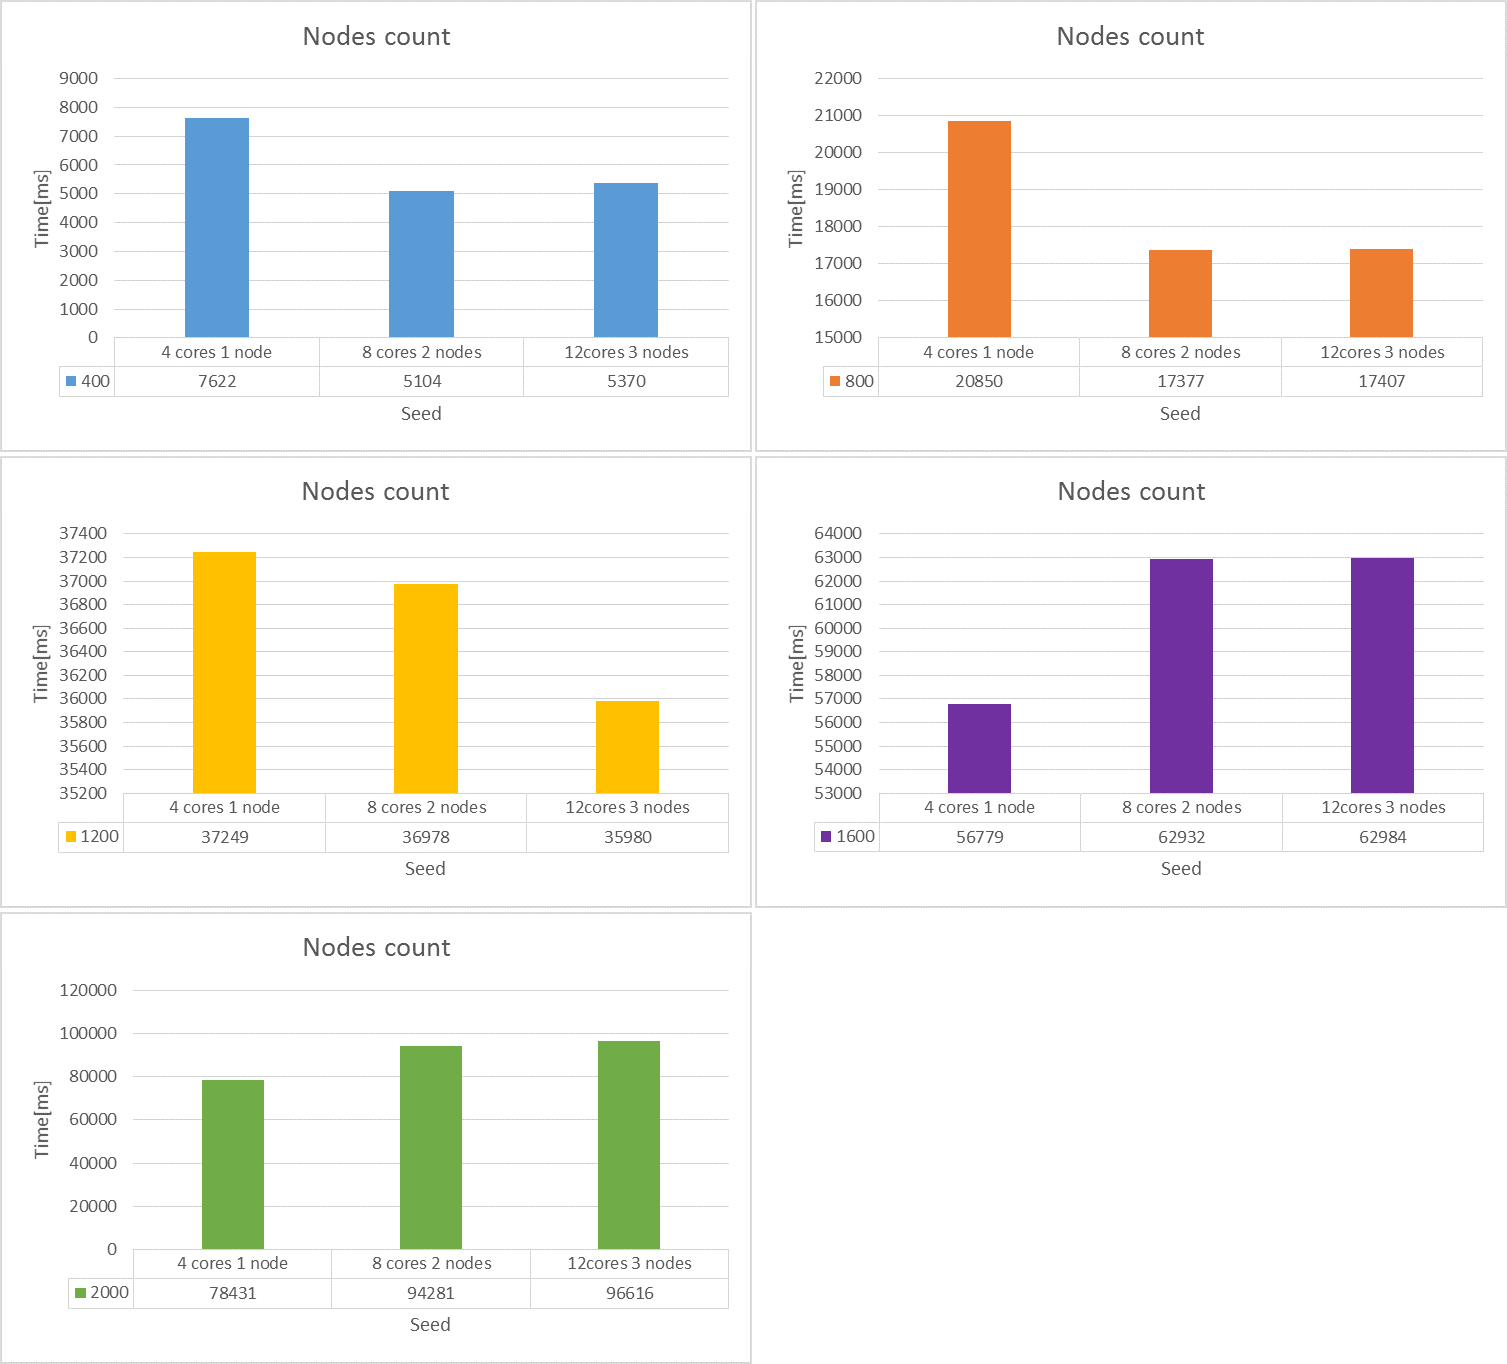
\includegraphics[width=\textwidth]{6.png}
    \caption{Porównanie czasu dla różnych rozmiarów klatek}
    \label{fig:my_frac}
\end{figure}

Na wykresach czasu trwania wykonania zadania od wielkości klatki w pikselach możemy zauważyć dwie tendencje dla czasu wykonania. Pierwsza z nich to spadkowa, jeśli zwiększamy ilość węzłów i jest ona zauważalna dla rozmiarów klatek 400, 800, 1200. Druga z nich to tendencja wzrostowa jeśli zwiększamy ilość węzłów i widać ją dla rozmiaru klatek 1600 i 2000. Tendencja spadkowa przy małych klatkach jest spowodowana zwiększeniem mocy obliczeniowej klastra. Natomiast tendencja wzrostowa wynika ze zbyt długiego czasu przesyłania wyniku do węzła master. W tym czasie inne węzły mogą ukończyć zadanie i niestety muszą czekać dłużej na swoją kolej obsługi. Drugim, dość oczywistym wnioskiem, jest to że im większy rozmiar klatki tym więcej czasu potrzeba na wykonanie zadania.

\section{Podsumowanie}
Otrzymane wyniki są dość niespodziewane. Wydawać by się mogło, że dodatkowe węzły liczące powinny powodować redukcję czasu potrzebnego na obliczenia. Tymczasem, nasze pomiary nie wykazują tej własności. Najprawdopodobniej użyty do łączenia maszyn interfejs FastEthernet ma zbyt małą przepustowość przez co procesory nie są maksymalnie wykorzystane i występuje długi czas oczekiwania na komunikację pomiędzy masterem i slavem.

Projekt ten ukazał zalety wynikające z rozpraszania obliczeń na wielu maszynach. Ponadto pokazał, jak używać technologii rozproszonych i webowych (MPI, frameworku Django, języka Python).

\newpage
\listoffigures
\addcontentsline{toc}{section}{Spis rysunków}

\end{document}